\chapter{Background Information - Cookies}
\label{ch:bg_cookies}
Intro sentence


%
% Section: Cookies
%
\section{Cookies}
\label{sec:bg_cookies:cookies}
Cookies are an easy way for websites to save the state or session of a user. In other words, cookies make it possible to create stateful web applications. This is done while browsing a website by sending information back and forth between the client and server. This information is saved as a simple text-file within the user's browser and contains a variety of arbitrary information. \cite{cookies1}

By saving cookies, the server knows details about the user's session such as who is currently logged in or what items are in the user's shopping cart. Thus, a user does not have to log in anew every time they visit the same website. With this information, a profile of the individual user is created and stored within the cookie. \cite{cookies1}



%
% Section: Tracking User Data
%
\section{Tracking User Data}
\label{sec:bg_cookies:data}
It is clear how information about a state or session can be saved in a browser, but how does that allow for third parties to identify and track the current user?

Third parties, such as Facebook or Google, are able to display personalized ads on the website a user is currently visiting by utilizing cookie syncing. With this method, domains assign an ID to a user, which is then passed between domains. \cite{cookies2}

textit{\color{red}Todo: Third party cookies}

%
% Section: Privacy and Policies
%
\section{Privacy and Policies}
\label{sec:bg_cookies:privacy}

Gathering users' information in ways that they are not aware of begs the question if this is legal and what policies exist in order to save users of unwanted tracking.

A study from 2009 showed that 66\% of Americans do not want to have targeted ads based on the information attained by being tracked. More so, when users were made aware of how the information was attained, 73\% - 86\% of users rejected personalized ads. \cite{americansRejectAds}

This study exemplifies that typical users do not want to have detailed information of them tracked and used for advertising. Tracking and labeling users in ways that they do not understand is deemed to be unethical. However, advertisers argue that this allows them to give users what they what: personalized advertisements rather than generic ones. \cite{americansRejectAds}

\begin{figure}[t]
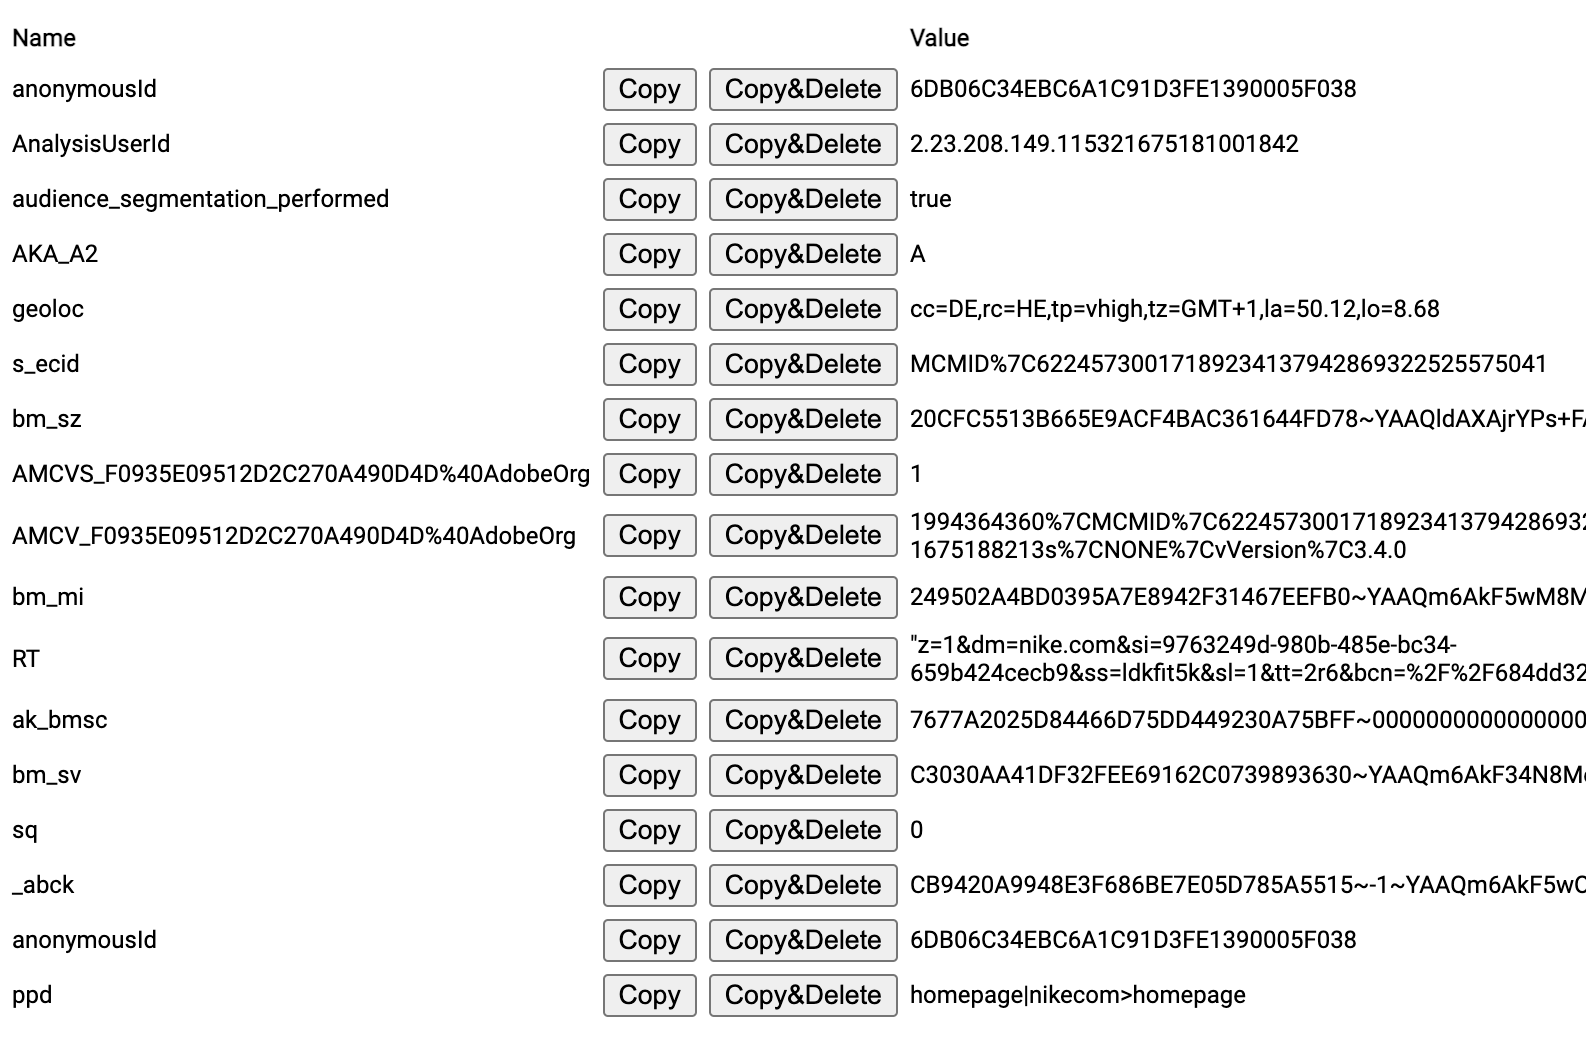
\includegraphics[width=\textwidth]{./gfx/cookiesScreenshot.png}
\centering
\caption{A screenshot of all active cookies being used when visiting \textit{https://www.nike.de}}
\label{fig:nikeCookies}
\end{figure}

\textit{\color{red}Todo: More on privacy, since this is one of the main reasons to look for alternatives. Can you find sources on how business models are being broken by privacy policies? Also describe how the screenshot has seemingly arbitrary content set in the cookies. It's encoded and can't be read, but contains a plethora of information.}
